\section{Linearisability testing}
\label{sec:lin-testing}

In the following two sections, we describe techniques for testing whether the
implementation of a synchronisation object is synchronisation linearisable
with respect to a synchronisation specification object.
%
Most of the techniques are influenced by the techniques for testing (standard)
linearisation~\cite{gavin:lin-testing}, so we begin by sketching those
techniques.

The idea of linearisability testing is as follows.  We run several threads,
performing operations (typically chosen randomly) upon the concurrent datatype
that we are testing, and logging the calls and returns.  More precisely, a
thread that performs a particular operation~$\sm{op}^i(x)$: (1) writes
$\call.\sm{op}^i(x)$ into the log; (2)~performs $\sm{op}(x)$ on the
synchonisation object, obtaining result~$y$, say; (3)~writes
$\return.\sm{op}^i \:: y$ into the log.  Further, the logging associates each
invocation with an invocation $\sm{op}(x)$ of the corresponding operation
on the specification object.

Once all threads have finished, we can use an algorithm to test whether the
history is linearisable with respect to the specification object.  Informally,
the algorithm searches for an order to linearise the invocations, consistent
with what is recorded in the log, and such that the order represents a legal
history of the corresponding invocations on the specification object.
See~\cite{gavin:lin-testing} for details of several algorithms.

This process can be repeated many times, so as to generate and analyse many
histories.  Our experience is that the technique works well.  It seems
effective at finding bugs, where they exist, typically within a few seconds;
for example, we used it to find an error in the concurrent priority queue
of~\cite{faulty-pri-queue}, which we believe had not previously been
documented.  Further, the technique is easy to use: we have taught it to
undergraduate students, who have used it effectively.

Note that this testing concentrates upon the safety property of linearisability,
rather than liveness properties such as deadlock-freedom.  However, if the
concurrent object can deadlock, it is likely that the testing will discover
this.  Related to this point, it is the responsibility of the tester to define
the threads in a way that all invocations will eventually return, so the
threads terminate.  For example, consider a partial stack where a |pop|
operation blocks while the stack is empty; here, the tester would need to
ensure that threads collectively perform at least as many |push|es as |pop|s,
to ensure that each |pop| does eventually return.

Note also that there is potentially a delay between a thread writing the
$\call$ event into the log and actually calling the operation; and likewise
there is potentially a delay between the operation returning and the thread
writing the $\return$ event into the log.  However, these delays do not
generate false errors: if a history without such delays is linearisable, then
so is a corresponding history with delays.  We believe that it is essential
that the technique does not give false errors: an error reported by testing
should represent a real error; testing of a correct implementation should be
able to run unsupervised, maybe for a long time.  Further, our experience is
that the delays do not prevent the detection of bugs when they exist (although
might require performing the test more times).  This means that a failure to
find any bugs, after a large number of tests, can give us good confidence in
the correctness of the concurrent datatype.

%% Note, assumes deterministic specification object. 

%%%%%%%%%%%%%%%%%%%%%%%%%%%%%%%%%%%%%%%%%%%%%%%%%%%%%%%

\section{Hacking the linearisablity framework}
\label{sec:testing-hacking}

%% Can we encode synchronisation linearisability within the linearisability
%% tester, using the correspondence of the previous section?  Jonathan to think
%% about this.  Will need to perform two log additions for some concrete
%% operations.

In this section we investigate how to use the existing linearisation testing
framework for testing synchronisation linearisation, using the ideas of
Section~\ref{sec:relating}.  This is not a use for which the framework
was intended, so we consider it a hack.  However, it has the advantage of not
requiring the implementation of any new algorithms.

Recall, from the introduction of Section~\ref{sec:relating}, that a
straightforward approach won't work.  Instead we adapt the idea of two-step
linearisation from later in that section.  We start by considering the case of
binary heterogeneous synchronisation.  We aim to obtain a log history that can
be tested for (standard) linearisability against |TwoStepLinSpec|.

As with standard linearisability testing, we run several threads, calling
operations on the synchronisation object, and logging the calls and returns. 
%
\begin{itemize}
\item A thread~$t$ that performs the concrete operation~$\op_1(x_1)$: (1)~writes
  $\call.\sm{op}_1^i(x_1)$ into the log, associating it with a corresponding
  invocation $\op_1(t, x_1)$ on the specification object; (2)~performs
  $\op_1(x_1)$ on the synchonisation object, obtaining result~$y_1$, say;
  (3)~writes $\return.\op_1^i \:: ()$ into the log; (4)~writes
  $\call.\overline{\op}_1^i()$ into the log, associating it with a
  corresponding invocation $\overline{\op}_1(t)$ on the specification object;
  (5)~writes $\return.\overline{\op}_1^i \:: y_1$ into the log.

\item A thread that performs operation~|op|\s2 acts as for standard
  linearisability testing.
\end{itemize}
%
%% Figure~\ref{fig:two-step-log} illustrates a possible log.
%


%%%%%

As with standard linearisation, the tester needs to define the
threads so that all invocations will eventually return, i.e.~that each will be
able to synchronise.  For a binary synchronisation with no precondition, we
can achieve this by half the threads calling one operation, and the other half
calling the other operation (with the same number of calls by each).

Once all threads have finished, we test whether the log history is
linearisable (i.e.~standard linearisation) with respect to |TwoStepLinSpec|
from Section~\ref{sec:relating}.
%
Note there might be delays involved in writing to the log, so that the log
history does not correspond precisely to the history of operation calls and
returns.  We show that the approximation serves our purposes.

%%  We refer to the \emph{log history}, to distinguish it from the history of
%% calls and returns on the synchronisation object.

Consider a history~$h$ of the synchronisation object, and suppose, for the
moment, there are no delays in logging, i.e.:\ (1)~the $\call.\op_1$ and
$\call.\op_2$ events happen immediately before the actual calls; (2)~the
$\return.\op_2$ events happen immediately after the return of~$\op_2$; and
(3)~the $\call.\overline\op_1$ and $\return.\overline\op_1$ events happen
immediately after the return of $\op_1$ --- in each case with no intervening
events.  Then the log history is linearisable with respect to |TwoStepLinSpec|
if and only if the history~$h$ is two-step linearisable with respect to
|TwoStepLinSpec|.  But Proposition~\ref{prop:two-step-lin} then shows that
this holds if and only if $h$ is synchronisation linearisable.  In particular,
this shows that errors are detected providing the logging is fast enough.

We now show that delays in logging do not introduce false errors.  Consider a
history~$h$ that is synchronisation linearisable, and consider the
corresponding log history~$h_l$.  Now build a history~$h'$ so that each
operation is extended so that: (1)~each call of~$\op_1$ or~$\op_2$ is
immediately before the $\call.\op_1$ or $\call.\op_2$ event in~$h_l$; (2)~each
return of~$\op_1$ is immediately after the $\return.\overline\op_1$ event
in~$h_l$; and (3)~each return of~$\op_2$ is immediately after the
$\return.\op_2$ event in~$h_l$.  This construction is illustrated below for
the two types of operation.
%
\begin{center}
\begin{tikzpicture}[xscale = 1.0, yscale = 1.0]
\draw (-2.0,0) node{$h$:};
\draw (-2.0,-1) node{$h_l$:};
\draw (-2.0,-2.3) node{$h'$:};
% op_1^1
\draw[|-|] (0,0) -- node[above] {$\sm{op}_1(x_1)\::y_1$} (1,0);
\bulletAt(-0.2,-0.8){$\call.\sm{op}_1$}
\bulletAt(1.2,-0.8){$\return.\sm{op}_1$}
\bulletAt(2.7,-0.8){$\call.\overline{\op}_1$}
\bulletAt(4.2,-0.8){$\return.\overline{\op}_1$}
\draw[|-|] (-0.4,-2.3) -- node[above] {$\sm{op}_1(x_1)\::y_1$} (4.4,-2.3);
%%%%%
\draw[|-|] (7.0,0) -- node[above] {$\sm{op}_2(x_2)\::y_2$} (8,0);
\bulletAt(6.8,-0.8){$\call.\sm{op}_2$}
\bulletAt(8.2,-0.8){$\return.\op_2$}
\draw[|-|] (6.6,-2.3) -- node[above] {$\sm{op}_2(x_2)\::y_2$} (8.4,-2.3);
\end{tikzpicture}
\end{center}
%
Now $h$ is synchronisation linearisable; and hence $h'$ is also (since each
operation in $h'$ is an extension of the corresponding operation in~$h$).  But
then Proposition~\ref{prop:two-step-lin} implies that $h'$ is two-step
linearisable with respect to |TwoStepLinSpec|.  Hence $h_l$ is linearisable
with respect to |TwoStepLinSpec|, by construction.

This approach generalises to non-binary synchronisations, homogeneous
synchronisations, and stateful specification objects as in
Section~\ref{ssec:relating-variations}.

%\framebox{Generalisations}

%%%%%%%%%%%%%%%%%%%%%%%%%%%%%%%%%%%%%%%%%%%%%%%%%%%%%%%

% \framebox{Improve below}

However, it is not, in general, possible to capture variable-arity
synchronisations where the arity depends upon the relative timing of
invocations, as opposed to the state of the specification object.  This is a
result of two things: that the logging of operations, in particular the
$\overline{\op}_1$, can be arbitrarily delayed; and that it can be
nondeterministic whether or not two invocations synchronise, which is at odds
with the fact that each operation on the specification object needs to be
deterministic.

To illustrate this point, consider a timeout channel.  Without loss of
generality, let the |send| operation correspond to $\op_1$, and the
|receive| operation correspond to~$\op_2$.

The left-hand side of Figure~\ref{fig:two-step-timeout-channel} gives a
timeline illustrating a successful |send(3)| and |receive|.  Note that this
corresponds to the history
\[
\seq{ \send(3)\::(),\; \receive()\::\sm{Some}(3),\; 
  \overline{\send}(3)\::\sm{true} }
\]
of the specification object.

%%%%%%%%%%

\begin{figure}
\begin{center}
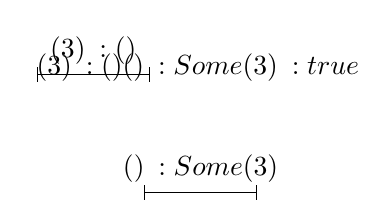
\begin{tikzpicture}[xscale = 0.9]
\draw[|-|] (0,0) -- node[above] {$\send(3)\::()$} (1.6,0);
\crossAt(0.7,0){$\send(3)\::()$}
%
\draw[|-|] (0.3,-1.5) -- 
  node[above] {$\receive()\::\sm{Some}(3)$} (1.9,-1.5);
\crossAt(1.5,-1.5){$\receive()\::\sm{Some}(3)$}
%
\draw[|-|] (2.5,0) -- node[above] 
  {$\overline{\send}(3)\::\sm{true}$} (4.1,0);
\crossAt(3.3,0){$\overline{\send}\::\sm{true}$}
%% \draw[|-|] (4,0) -- 
%%   node[above] {$\overline{\sendWithin}(3)\::\sm{true}$} (6,0);
%
%\draw (0,-2.5) -- (7.5,-2.5);
\end{tikzpicture}
%%%%%%
\hfil\hfil
%\bigskip
\begin{tikzpicture}[xscale = 0.9]
\draw[|-|] (0,-3.5) -- node[above] {$\send(3)\::()$} (1.6,-3.5);
\crossAt(0.7,-3.5){$\send(3)\::()$}
%
\draw[|-|] (2.2,-5) -- 
  node[above] {$\receive()\::\sm{None}$} (3.8,-5);
\crossAt(3.4,-5){$\receive()\::\sm{Some}(3)$}
%
\draw[|-|] (4.0,-3.5) -- node[above] 
  {$\overline{\send}(3)\::\sm{false}$} (5.6,-3.5);
\crossAt(4.8,-3.5){$\overline{\send}(3)\::\sm{true}$}
%% \draw[|-|] (5.5,-3.5) -- 
%%   node[above] {$\overline{\sendWithin}(3)\::\sm{false}$} (7.5,-3.5);
\end{tikzpicture}
\end{center}
\caption{Figure showing why two-step linearisation cannot be used for a
  timeout channel.  The horizontal lines and the labels above represent the
  log history; the crosses and the labels below illustrate the linearisation
  points.  For simplicity, we omit invocation identifiers and thread
  identities.}
\label{fig:two-step-timeout-channel}
\end{figure}

%%%%%%%%%%

The right-hand side of Figure~\ref{fig:two-step-timeout-channel} gives a
timeline illustrating an unsuccessful |send(3)| and |receive|, and where the
logging of $\overline{\send}$ is delayed.  None of the invocations overlap, so
they must necessarily be linearised in the same order as in the previous
history.  The specification object is deterministic, so the operations must
return the same results as in the previous history.  But, in the cases of
$\receive$ and $\overline{\send}$, those returned values do not agree with the
corresponding values in the log history.  Hence the history would be flagged
as an error, despite being valid.

The difference between this situation and the discussion in
Section~\ref{ssec:relating-variations} concerns the fact that the logging of
operations, in particular the $\overline{\send}$, can be arbitrarily delayed.
However, in the earlier section we allowed the $\overline{\send}$ anywhere
within the corresponding concrete operation.  This means that a history like
in Figure~\ref{fig:two-step-timeout-channel} (right) could be linearised by
the history
\[
\seq{ \send(3)\::(),\; \overline{\send}(3)\::\sm{false},\;
  \receive()\::\sm{None} }
\]
of the specification, where the operations take place in a different order
than for Figure~\ref{fig:two-step-timeout-channel}; this is consistent with a
deterministic specification object.
